\documentclass[border=1cm]{standalone}
\usepackage{tikz}

% Рекурсивный макрос: ковёр Серпинского
\newcommand{\carpet}[4]{%
  % #1 x, #2 y, #3 size, #4 depth
  \ifnum#4=0
    \fill (#1,#2) rectangle ++(#3,#3);
  \else
    \pgfmathsetmacro{\s}{#3/3}
    \foreach \i in {0,1,2} {
      \foreach \j in {0,1,2} {
        \ifnum\i=1\relax
          \ifnum\j=1\relax
            % центральный квадрат пропускаем
          \else
            \carpet{#1+\i*\s}{#2+\j*\s}{\s}{\numexpr#4-1\relax}
          \fi
        \else
          \carpet{#1+\i*\s}{#2+\j*\s}{\s}{\numexpr#4-1\relax}
        \fi
      }
    }
  \fi
}

\begin{document}
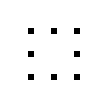
\begin{tikzpicture}

% старт: x y size depth
\carpet{0}{0}{6}{4}

\end{tikzpicture}
\end{document}
